\section{Introduction}

\begin{frame}
  \frametitle{High Performance Computing}
  \begin{columns}
    \column{.5\textwidth}
    \begin{center}
      \begin{figure}
        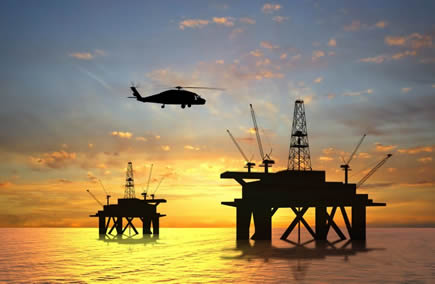
\includegraphics[scale=0.2]{figs/oil-gas-industry.jpg}\\
        \caption{Oil and Gas}
      \end{figure}
      \begin{figure}
        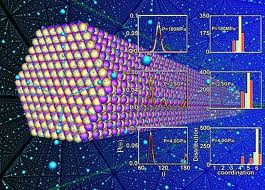
\includegraphics[scale=0.3]{figs/scientific-computing.jpg}\\
        \caption{Scientific Computing}
      \end{figure}
    \end{center}
    \column{.5\textwidth}
    \begin{center}
      \begin{figure}
        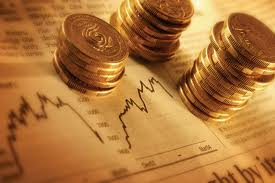
\includegraphics[scale=0.31]{figs/finance.jpg}\\
        \caption{Finance}
      \end{figure}
      \begin{figure}
        
\includegraphics[scale=0.31]{figs/ads.jpg}\\
        \caption{Online Advertising}
      \end{figure}
    \end{center}
  \end{columns}
\end{frame}

\begin{frame}
  \frametitle{High Performance Computing}
  \begin{beamerboxesrounded}{Goals}
    HPC software must to be:
    \begin{itemize}
      \item fast
      \item energy efficient
      \item easy to develop and maintain
    \end{itemize}
    \end{beamerboxesrounded}
    \vspace{0.75cm}
  \begin{beamerboxesrounded}{This Project}
    Investigates more efficient and more productive HPC solutions using
    dataflow engines and aspect-oriented programming.
  \end{beamerboxesrounded}
\end{frame}

\begin{comment}
\begin{frame}[fragile]
  \frametitle{HPC: The CPU Way}
  \begin{lstlisting}
    for (int i = 0; i < n; i++)
    sum+=x[i]
  \end{lstlisting}
  \begin{lstlisting}
    some assembly
  \end{lstlisting}
\end{frame}
\end{comment}

\begin{frame}
  \frametitle{HPC: The Dataflow Way}
  \begin{figure}[!ht]
    \centering
    \def\svgwidth{0.7\linewidth}
    \input{figs/dataflow-graph.pdf_tex}
  \end{figure}
\end{frame}

\begin{frame}
  \frametitle{HPC: The Dataflow Way}
  Run-time environment -- MaxWorkstation
  \begin{figure}[!ht]
    \centering
    \def\svgwidth{\linewidth}
    \input{figs/max-workstation.pdf_tex}
  \end{figure}
\end{frame}


\begin{frame}
  \frametitle{CPU vs Dataflow}
  \begin{columns}
    \begin{column}{.5\linewidth}
      \begin{figure}[!ht]
        \centering
        \def\svgwidth{\linewidth}
        \input{figs/compute-cpu.pdf_tex}
      \end{figure}
      \begin{itemize}
      \item Fast to develop
      \item Inefficient
      \end{itemize}
    \end{column}
    \begin{column}{.5\linewidth}
      \begin{figure}[!ht]
        \centering
        \def\svgwidth{\linewidth}
        \input{figs/compute-dfe.pdf_tex}
      \end{figure}
      \begin{itemize}
      \item Slow to develop
      \item Efficient
      \end{itemize}
    \end{column}
  \end{columns}
\end{frame}

\begin{frame}[fragile]
  \frametitle{Kernel Optimisations: Bit Width}
      \begin{figure}[!ht]
        \centering
        \def\svgwidth{.7\linewidth}
        \input{figs/dfg-cast.pdf_tex}
      \end{figure}
\end{frame}

\begin{frame}[fragile]
  \frametitle{Kernel Optimisations: Stream Pipelineing}
      \begin{figure}[!ht]
        \centering
        \def\svgwidth{.7\linewidth}
        \input{figs/dfg-pipeline.pdf_tex}
      \end{figure}
\end{frame}

\begin{frame}[fragile]
  \frametitle{Kernel Optimisations: Pipeline Replication}
      \begin{figure}[!ht]
        \centering
        \def\svgwidth{.7\linewidth}
        \input{figs/dfg-parallel.pdf_tex}
      \end{figure}
\end{frame}

\begin{frame}[fragile]
  \frametitle{A Typical Dataflow Kernel: RTM}
  \begin{itemize}
    \item RTM - Reverse Time Migration for seismic imaging
    \item MaxJ - Java API for dataflow programming with FPGAs
  \end{itemize}

  \begin{lstlisting}
// I/O type
KArrayType burstIn = new KArrayType(hwFloat(8,24), Par);

// Compute type
for (int i = 0; i < Par; i++)
  source[i] = burstIn[i].cast(hwFloat(8, 22));

// Optimisations
optimization.pushDSPFactor(1);

// Pipeline replication
for (int i = 0; i < Par; i++)
  result[i][0] = cur[0][6+i][5][5] * 2.0 - (...)
\end{lstlisting}
\end{frame}

\begin{frame}[fragile]
  \frametitle{Issues}
  Have to:
  \begin{enumerate}

    \item specify I/O type and width to interface with host API
    \item minimise compute type width to optimise resource usage
    \item specify casting between types to ensure correct values
    \end{enumerate}

\begin{lstlisting}
  // IOType
  KArrayType burstIn = new KArrayType((*@\reduline{hwFloat(8, 24)}@*), (*@\reduline{Par}@*));

  // Compute Type
  for (int i = 0; i < Par; i++)
    source[i] = burstIn[i].(*@\reduline{cast(hwFloat(8, 22))}@*);
  \end{lstlisting}
\end{frame}

\begin{frame}[fragile]
  \frametitle{Issues}
  Have to:
  \begin{enumerate}
    \setcounter{enumi}{4}
      \item apply FPGA specific optimisations
      \item apply per stream or per block optimisation function calls
      \end{enumerate}
    \begin{lstlisting}
// Map arithmetic to Digital Signal Processors
optimization.pushDSPFactor(1);
{ /* compute block */ }
optimization.popDSPFactor();

// Add pipeline registers to stream (improve timing)
optimization.pipeline(stream);

    \end{lstlisting}
\end{frame}

\begin{frame}[fragile]
  \frametitle{Issues}
    \begin{beamerboxesrounded}{The Problem}
      Mixing optimisations with application code:
      \begin{itemize}
        \item harder to infer
        \item harder to automate
        \item less portable (cannot apply to other applications)
      \end{itemize}
    \end{beamerboxesrounded}
    \begin{beamerboxesrounded}{The Solution}
      Decouple optimisations from application code:
    \begin{itemize}
    \item infer information as much as possible
    \item encapsulate optimisations in separate modules
    \item apply them automatically to explore the design space
    \end{itemize}
    \end{beamerboxesrounded}
\end{frame}
